%!TEX root = ../../../../memoria.tex
\subsection{\ecomFrameworkCoreEF}

Corresponde a la customización de los elementos relacionados directamente con la tienda. La información se ha jerarquizado en diferentes paneles de contenido plegable (conocidos como menú acordeón) los cuales se observan en la \refFigura{figure:dashboard:ecommerce:main_menu}.
%Displays collapsible content panels for presenting information in a limited amount of space.
\begin{figure}[H]
	\centering
	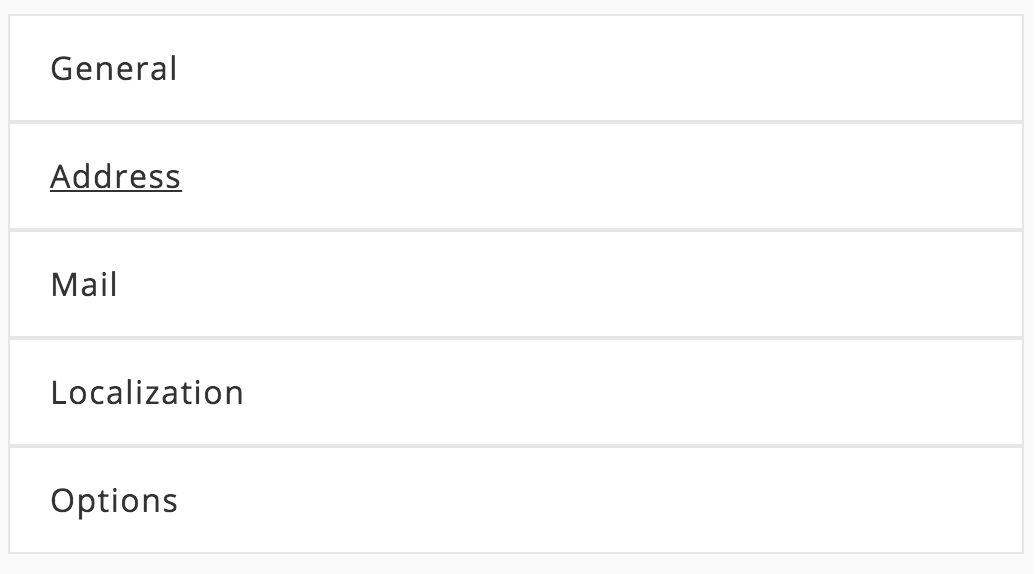
\includegraphics[width=0.6\textwidth]{figuras/dashboard/ecommerce/main_menu.png}
	\caption{Menú general de \ecomFrameworkCoreEF.}
	\label{figure:dashboard:ecommerce:main_menu}
\end{figure}

Cada uno de estos elementos tiene información configurable, además del \feedback habitual correspondiente a la información entregada de validación de cada campo, tiene una ventana emergente para indicar si la actualización del formulario fue o no exitosa.
La rázon de esta información extra es muy sencilla, si no existieran estos mensajes emergentes, estaría la ambigüedad de si el resultado fue exitoso o no dado que no hay ningún otro elemento gráfico con el cual se podría inferir el resultado. Por ejemplo, el formulario no se \'limpia\', el formulario no se cierra, no se agrega un nuevo elemento a una lista, etc.

\begin{figure}[H]
	\centering
	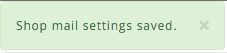
\includegraphics[width=0.6\textwidth]{figuras/dashboard/ecommerce/success_message.png}
	\caption{Mensaje de confirmación de éxito en la actualización del formulario. Este mensaje se esconde después de un breve intervalo de tiempo.}
	\label{figure:dashboard:ecommerce:success_message}
\end{figure}

\begin{figure}[H]
	\centering
	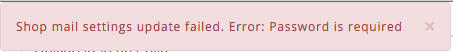
\includegraphics[width=0.8\textwidth]{figuras/dashboard/ecommerce/error_message.png}
	\caption{Mensaje para informar sobre un error en el proceso de actualización del formulario.}
	\label{figure:dashboard:ecommerce:error_message}
\end{figure}

En el caso de ser exitoso, aparece un mensaje el cual eventualmente desaparecerá de un breve intervalo de tiempo(\refFigura{figure:dashboard:ecommerce:success_message}). Los mensajes de error persisten en el tiempo. Por lo tanto se deben cerrar para que desaparezcan (\refFigura{figure:dashboard:ecommerce:error_message}).


\subsubsection*{Panel \generalPanel}

El panel general está formado por dos formularios; el primero solo contiene un campo y es un checkbox para permitir que un usuario \userGuestAccount pueda realizar un \checkoutCOM (\refFigura{figure:dashboard:ecommerce:general_menu:allow_checkout}).

\begin{figure}[H]
	\centering
	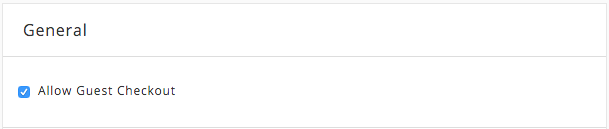
\includegraphics[width=0.6\textwidth]{figuras/dashboard/ecommerce/general_menu/allow_checkout.png}
	\caption{Formulario de información general de la tienda}
	\label{figure:dashboard:ecommerce:general_menu:allow_checkout}
\end{figure}

Este formulario tiene la particuladidad que se envía automáticamente al cambiar su estado.
El otro formulario está relacionado con la información más general de la empresa ( \refFigura{figure:dashboard:ecommerce:general_menu:menu})

\begin{figure}[H]
	\centering
	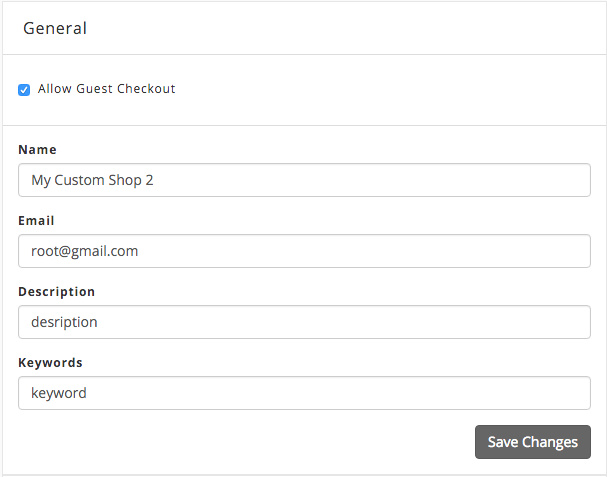
\includegraphics[width=0.6\textwidth]{figuras/dashboard/ecommerce/general_menu/menu.png}
	\caption{Formulario de información general de la tienda}
	\label{figure:dashboard:ecommerce:general_menu:menu}
\end{figure}

\begin{table}[H]
    \centering
	\begin{tabular}{ |l|c||l| }
		\hline Campo & Requerido & Restricción \\ \hline
		\multirow{1}{*}{\textit{Name}} 			&  {\checkmark} &  \\ \hline
		\multirow{1}{*}{\textit{Email}} 		&  				&  Debe ser un email válido.\\ \hline
		\multirow{1}{*}{\textit{Description}} 	&  				&  \\ \hline
		\multirow{1}{*}{\textit{Keywords}} 		&  				&  \\ \hline
		\hline
	\end{tabular}
 	\caption{Restrincciones formulario \generalPanel}
    \label{tab:dashboard:ecommerce:form:general}
\end{table}


Este formulario solo tienen un campo obligatorio, y corresponde a \textit{Name}. Al igual que otros formularios, dicho campo se destaca de color rojo, además de entregar un mensaje a modo de identificar el error (\refFigura{figure:apendice:dashboard:ecommerce:general_menu:updated_error}).



\subsubsection*{Panel \addressPanel}\label{capitulo:solucionImplementada:dashboard:subsubsection:addressPanel}

Este formulario se utiliza para agragar información física de la tienda, como algún teléfono de contacto.

\begin{figure}[H]
	\centering
	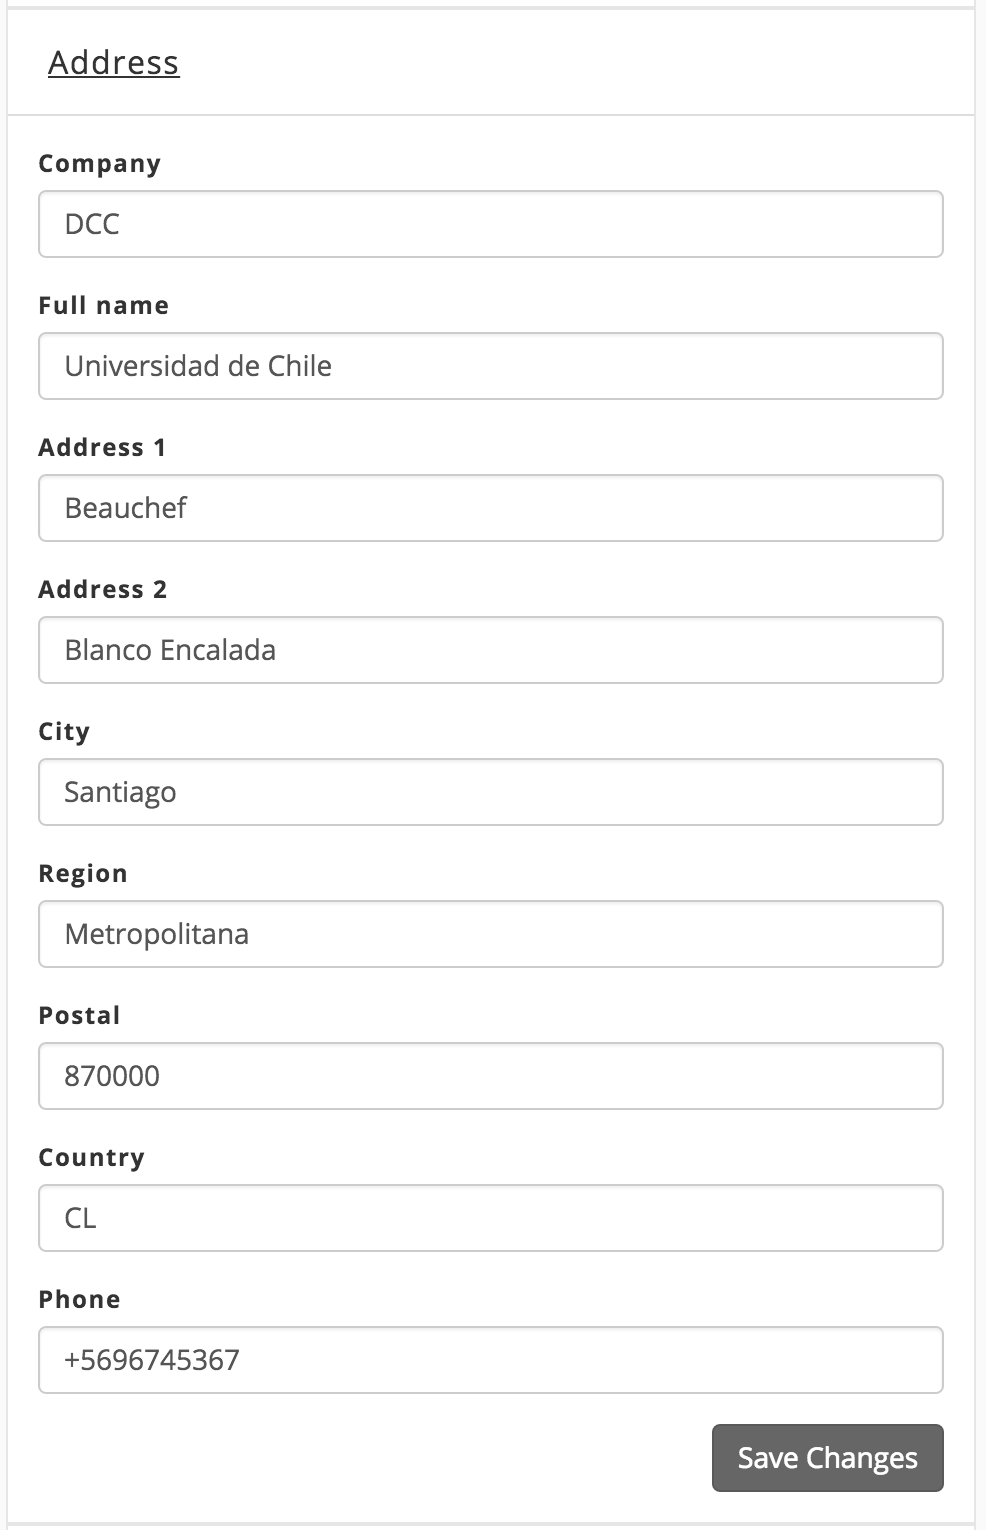
\includegraphics[width=0.5\textwidth]{figuras/dashboard/ecommerce/address/menu.png}
	\caption{Formulario de la dirección física de la tienda.}
	\label{figure:dashboard:ecommerce:address:menu}
\end{figure}

En relación a los campos del formulario, se tienen las siguientes restricciones (\reftabla{tab:dashboard:ecommerce:form:address}):

\begin{table}[H]
    \centering
	\begin{tabular}{ |l|c||l| }
		\hline Campo & Requerido & Restricción \\ \hline
		\multirow{1}{*}{\textit{Full name}} &  {\checkmark} &  \\ \hline
		\multirow{1}{*}{\textit{Address 1}} &  {\checkmark} &  \\ \hline
		\multirow{1}{*}{\textit{Address 2}} &   			&  \\ \hline
		\multirow{1}{*}{\textit{City}} 		&  {\checkmark} &  \\ \hline
		\multirow{1}{*}{\textit{Region}} 	&  {\checkmark} &  \\ \hline
		\multirow{1}{*}{\textit{Postal}} 	&  {\checkmark} &  \\ \hline
		\multirow{1}{*}{\textit{Country}}	&  {\checkmark} &  \\ \hline
		\multirow{1}{*}{\textit{Phone}} 	&  {\checkmark} &  \\ \hline
	\end{tabular}
 	\caption{Restrincciones formulario \addressPanel}
    \label{tab:dashboard:ecommerce:form:address}
\end{table}


\subsubsection*{Panel \mailPanel}

Corresponde a la información básica necesaria para configurar un servicio de \email. Agregar un \email no es requerido, pero si se configura el servicio deben agregarse tódos los campos(\reftabla{tab:dashboard:ecommerce:form:mail}).

\begin{figure}[H]
	\centering
	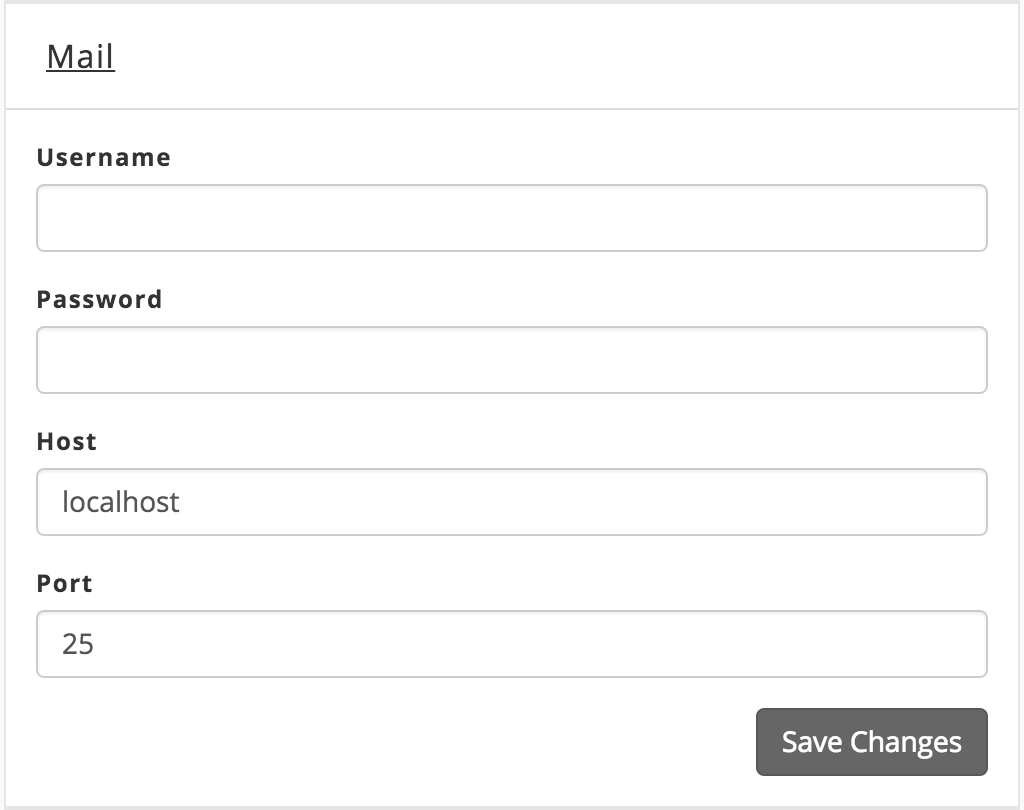
\includegraphics[width=0.6\textwidth]{figuras/dashboard/ecommerce/mail/menu.png}
	\caption{Formulario con la información de la configuración del Mail.}
	\label{figure:dashboard:ecommerce:mail:menu}
\end{figure}

\begin{table}[H]
    \centering
	\begin{tabular}{ |l|c||l| }
		\hline Campo & Requerido & Restricción \\ \hline
		\multirow{1}{*}{\textit{User Name}} &  {\checkmark} &  \\ \hline
		\multirow{1}{*}{\textit{Password}} 	&  {\checkmark} &  \\ \hline
		\multirow{1}{*}{\textit{Host}} 		&  {\checkmark} &  \\ \hline
		\multirow{1}{*}{\textit{Port}} 		&  {\checkmark} & Número mayor que 0 \\ \hline
		\hline
	\end{tabular}
 	\caption{Restrincciones formulario \mailPanel}
    \label{tab:dashboard:ecommerce:form:mail}
\end{table}


\subsubsection*{Panel \optionsPanel}

\begin{figure}[H]
	\centering
	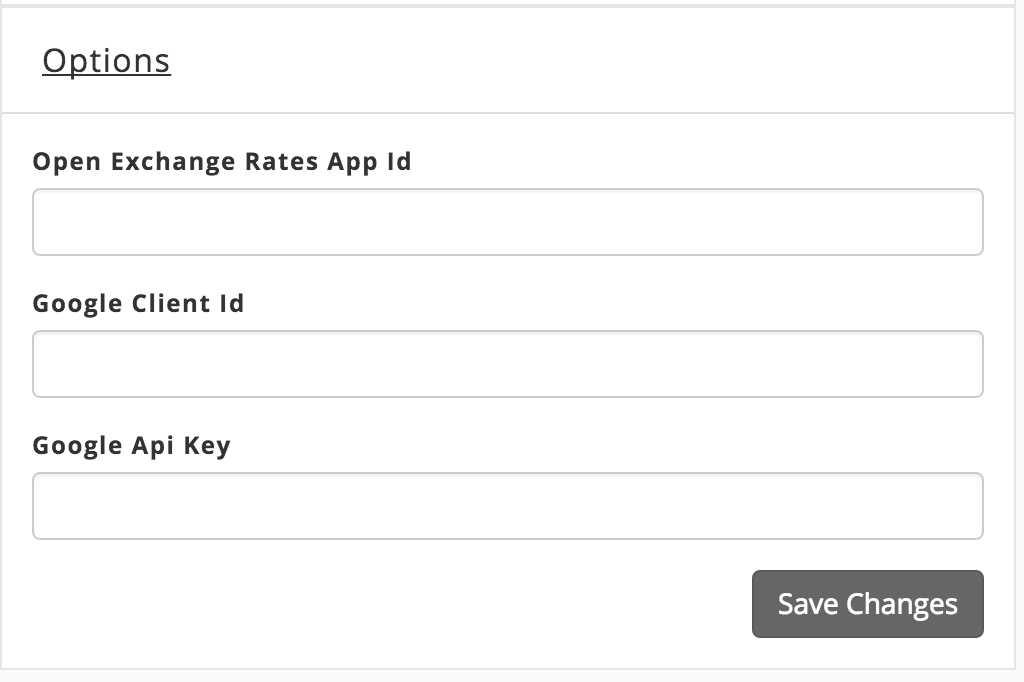
\includegraphics[width=0.6\textwidth]{figuras/dashboard/ecommerce/options/menu.png}
	\caption{Formulario con información relacionada con los Analytics.}
	\label{figure:dashboard:ecommerce:options:menu}
\end{figure}

\begin{table}[H]
    \centering
	\begin{tabular}{ |l|c||l| }
		\hline Campo & Requerido & Restricción \\ \hline
		\multirow{1}{*}{\textit{Open Exchange}} 	&  {\checkmark} &  \\ \hline
		\multirow{1}{*}{\textit{Google Client}} 	&  {\checkmark} &  \\ \hline
		\multirow{1}{*}{\textit{Google Api}} 		&  {\checkmark} &  \\ \hline
		\hline
	\end{tabular}
 	\caption{Restrincciones formulario \optionsPanel}
    \label{tab:dashboard:ecommerce:form:options}
\end{table}